% Fig 1 (fig:architecture): standalone source for the paper figure.
% Build: pdflatex architecture.tex  ->  architecture.pdf  (see build_figures.sh)
\documentclass[border=2pt]{standalone}
\usepackage[T1]{fontenc}
\usepackage{amsmath,amssymb}
\usepackage{tikz}
\usetikzlibrary{shapes.geometric, arrows.meta, positioning, patterns, calc}
% Okabe-Ito colorblind-safe palette (Wong 2011, Nature Methods)
\definecolor{oiblue}{HTML}{0072B2}
\definecolor{oiorange}{HTML}{E69F00}
\definecolor{oiskyblue}{HTML}{56B4E9}
\definecolor{oigray}{HTML}{999999}
\definecolor{oivermillion}{HTML}{D55E00}
\definecolor{oigreen}{HTML}{009E73}
\definecolor{oipurple}{HTML}{CC79A7}
\begin{document}
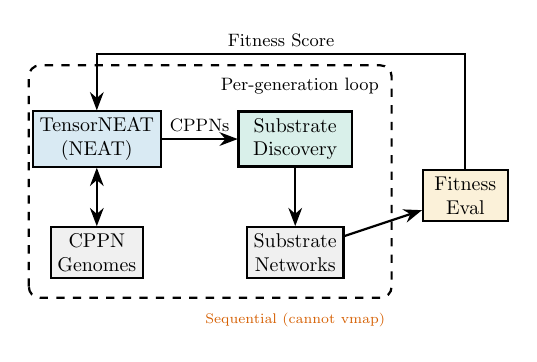
\begin{tikzpicture}[scale=0.72, every node/.style={scale=0.72},
    box/.style={rectangle, draw, thick, minimum width=2cm, minimum height=0.8cm, align=center},
    arrow/.style={-{Stealth}, thick}
]
    \node[box, fill=oiblue!15] (neat) at (0,2) {TensorNEAT\\(NEAT)};
    \node[box, fill=oigreen!15] (substrate) at (3.5,2) {Substrate\\Discovery};
    \node[box, fill=oigray!15, minimum width=1.5cm] (cppn) at (0,0) {CPPN\\Genomes};
    \node[box, fill=oigray!15, minimum width=1.5cm] (nets) at (3.5,0) {Substrate\\Networks};
    \node[box, fill=oiorange!15, minimum width=1.5cm] (fit) at (6.5,1) {Fitness\\Eval};
    \draw[arrow] (neat) -- (substrate) node[midway, above, font=\small] {CPPNs};
    \draw[{Stealth}-{Stealth}, thick] (neat) -- (cppn);
    \draw[arrow] (substrate) -- (nets);
    \draw[arrow] (nets) -- (fit);
    \draw[arrow] (fit) -- ++(0,2.5) -| (neat) node[pos=0.25, above, font=\small] {Fitness Score};
    \draw[dashed, thick, rounded corners] (-1.2,-0.8) rectangle (5.2,3.3);
    \node[font=\small, anchor=north east] at (5.1,3.2) {Per-generation loop};
    \node[font=\scriptsize, text=oivermillion] at (3.5,-1.2) {Sequential (cannot vmap)};
\end{tikzpicture}
\end{document}
